\begin{tikzpicture}
    % Definir los puntos del cuadrado
    \tkzDefPoint(0,0){A}
    \tkzDefPoint(4,0){B}
    \tkzDefPoint(4,4){C}
    \tkzDefPoint(0,4){D}

    % Dibujar el cuadrado
    \tkzDrawPolygon(A,B,C,D)

    % Marcar un lado
    \tkzLabelSegment[below](A,B){$l$}
    \tkzLabelSegment[right](B,C){$l$}

    % Marcar los puntos
    \tkzLabelPoints[below](A,B)
    \tkzLabelPoints[above](C,D)
\end{tikzpicture}